\begin{frame}
  \titlepage
\end{frame}

\begin{frame}{목차}
  \tableofcontents
\end{frame}

\section{Chapter 1: Getting Started with Graph Learning}

\begin{frame}{왜 그래프인가?}
\begin{itemize}
  \item 그래프는 노드(객체)와 엣지(관계)를 함께 모델링
  \begin{itemize}
    \item 노드: 엣지 없는 노드는 전통적인 데이터 표현으로도 가능
    \item 엣지: 반드시 2개 이상의 노드 포인트를 포함하며 관계 정보를 표현
  \end{itemize}
  \item 관계 정보가 핵심인 도메인에서 강력
  \item 예: 소셜/교통/생물/추천 시스템
  \item GNN: 관계 구조를 활용한 딥러닝 모델링 프레임워크
\end{itemize}

\end{frame}

\begin{frame}{Left: 노드 중심 표현, Right: 관계 중심 표현 (그래프)}

\centering
\IfFileExists{images/ch01_fig13_family_tree_tabular_vs_graph.png}{%
  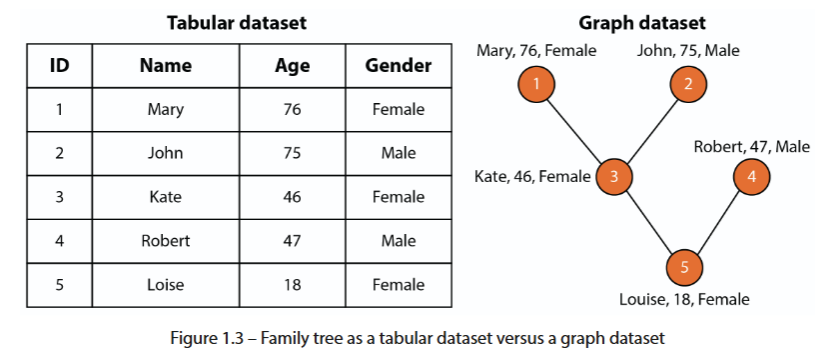
\includegraphics[width=0.93\linewidth]{images/ch01_fig13_family_tree_tabular_vs_graph.png}
}{%
  \fbox{\parbox{0.9\linewidth}{\centering
  이미지 파일을 추가하세요:\\
  \texttt{images/ch01\_fig13\_family\_tree\_tabular\_vs\_graph.png}}}
}

\end{frame}

\begin{frame}{관계 정보(엣지)의 테이블 표현}
\begin{columns}[T,onlytextwidth]
\begin{column}{0.49\textwidth}
\textbf{Node Table}
\vspace{0.2em}
\small
\begin{tabular}{llll}
\toprule
node\_id & name & age & gender \\
\midrule
1 & Mary & 76 & Female \\
2 & John & 75 & Male \\
3 & Kate & 46 & Female \\
4 & Robert & 47 & Male \\
5 & Loise & 18 & Female \\
\bottomrule
\end{tabular}
\end{column}
\begin{column}{0.49\textwidth}
\textbf{Edge Table}
\vspace{0.2em}
\small
\begin{tabular}{lll}
\toprule
edge\_id & src\_node\_id & dst\_node\_id \\
\midrule
1 & 1 & 3 \\
2 & 2 & 3 \\
3 & 3 & 5 \\
4 & 4 & 5 \\
\bottomrule
\end{tabular}
\vspace{0.35em}
\scriptsize
\begin{itemize}
  \item 엣지 한 행은 반드시 두 노드를 가리키는
  \texttt{src\_node\_id}, \texttt{dst\_node\_id} \textbf{두 포인터}를 가진다.
  \item 또한 연결 자체에 대한 별도의 정보를 가질 수 있다. (예: weight, relation category 등)
\end{itemize}
\end{column}
\end{columns}
\end{frame}

\begin{frame}{Graph Learning의 대표 과제}
\small
\begin{itemize}
  \item \textbf{Node Classification}: 각 노드의 라벨(클래스)을 예측
  \item \textbf{Link Prediction}: 두 노드 사이의 연결 존재 여부를 예측
  \item \textbf{Graph Classification}: 그래프 전체(분자/문서/세션)에 대한 라벨을 예측
  \item \textbf{Graph Generation}: 조건을 만족하는 새로운 그래프 구조를 생성
\end{itemize}
\vspace{0.3em}
\footnotesize
예: 사용자 관심사 분류(Node), 친구 추천(Link), 분자 독성 분류(Graph), 신규 분자 설계(Generation)
\end{frame}

\begin{frame}{GNN의 구조}
  \begin{columns}
    \begin{column}{0.5\textwidth}
      \begin{itemize}
        \item 입력: 그래프 구조 데이터
        \item GNN은 노드 특징과 관계 구조를 함께 활용해 표현 학습
        \item 출력: 노드/엣지/그래프 수준의 예측 등 문제 유형에 따라 다양한 태스크 수행
      \end{itemize}
    \end{column}
    \begin{column}{0.5\textwidth}
      \begin{center}
        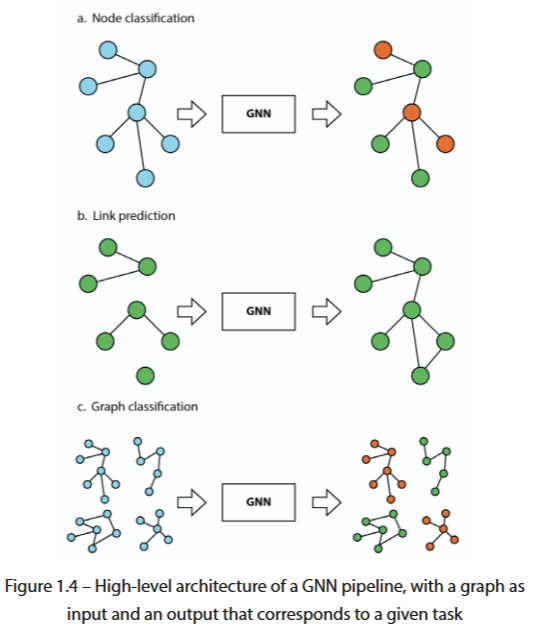
\includegraphics[height=0.8\textheight]{images/gnn_pipeline.png}
      \end{center}
    \end{column}
  \end{columns}
\end{frame}

\begin{frame}{문제 1: Node Classification}

\begin{center}
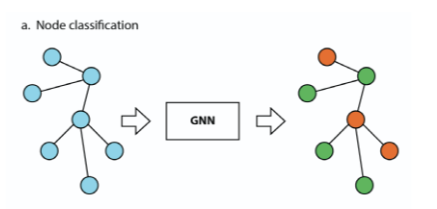
\includegraphics[height=0.5\textheight]{images/node_classification.png}
\end{center}

목표: 각 노드의 라벨을 예측

예시

\begin{itemize}
\item SNS 사용자 분류 - 예: 관심사/성향/스팸 여부
\item 논문 주제 분류 - 예: AI/시스템/이론 등
\item 금융 네트워크에서 사기 계좌 탐지 - 예: 정상/사기 계좌
\end{itemize}

\end{frame}

\begin{frame}{문제 2: Link Prediction}

\begin{center}
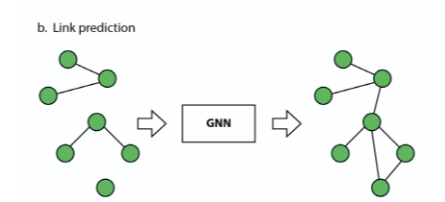
\includegraphics[height=0.5\textheight]{images/link_prediction.png}
\end{center}

목표: 아직 링크가 없는 두 노드 사이의 링크가 생길 가능성 예측

활용 예시

\begin{itemize}
\item SNS 친구 추천 - 예: A와 B가 친구가 될 가능성
\item 연구자 협업 예측 - 예: 연구자 A와 B가 공동 연구할 가능성
\item 추천 시스템 - 예: 사용자 A가 상품 B를 구매할 가능성
\end{itemize}

\end{frame}

\begin{frame}{문제 3: Graph Classification}

\begin{center}
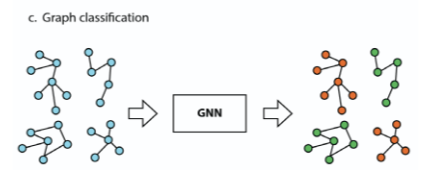
\includegraphics[height=0.5\textheight]{images/graph_classification.png}
\end{center}

목표: 그래프 전체에 대한 라벨 예측 - 그래크 전체를 하나의 객체로 보고 특정 태스크 수행

활용 예시

\begin{itemize}
\item 분자 구조의 독성 예측 - 예: 분자 A가 독성이 있는지 여부
\item 화합물의 약효 예측 - 예: 화합물 A가 특정 질병에 효과가 있는지 여부
\item 프로그램 코드 분석 - 예: 코드 A가 버그가 있는지 여부
\end{itemize}

\end{frame}

\begin{frame}{Graph Learning이 빠르게 발전한 이유}
\begin{itemize}
  \item 그래프 학습은 다양한 도메인에 적용 가능해 연구/개발 가치가 큼
  \item 최근 발전의 핵심 동력:
  \begin{itemize}
    \item 대규모 데이터셋 가용성 증가
    \item 고성능 컴퓨팅 자원 확장
    \item ML/AI 방법론의 빠른 발전
  \end{itemize}
\end{itemize}
\vspace{0.3em}
\textbf{대표 기술 계열 4가지}
\begin{enumerate}
  \item Graph Signal Processing
  \item Matrix Factorization
  \item Random Walk
  \item Deep Learning
\end{enumerate}
\end{frame}

\begin{frame}{4가지 Graph Learning Technique Family}
\small
\begin{itemize}
  \item \textbf{Graph Signal Processing}: 그래프 푸리에 변환/스펙트럴 분석으로 연결 구조의 내재 특성을 분석
  \item \textbf{Matrix Factorization}: 큰 관계 행렬을 저차원 잠재 표현으로 분해해 패턴을 compact하게 표현
  \item \textbf{Random Walk}: 그래프 위 탐색 경로를 시뮬레이션해 노드 간 관계 정보를 수집하고 학습 데이터 생성
  \item \textbf{Deep Learning}: 다층 신경망으로 그래프를 벡터로 인코딩해 다양한 다운스트림 과제에서 높은 성능 달성
\end{itemize}
\vspace{0.3em}
\footnotesize
실무에서는 이 기법들이 서로 배타적이라기보다, 혼합되어 함께 사용되는 경우가 많다.
\end{frame}

\begin{frame}{왜 GNN인가?}
\begin{itemize}
  \item 이웃 정보를 반복 집계(message passing)
  \item 노드 특징 + 관계 구조를 함께 반영
  \item 대규모/고복잡도 문제에서 표현학습에 유리
\end{itemize}
\[
h_v^{(k)} = \phi\!\left(h_v^{(k-1)},\;\bigoplus_{u\in\mathcal{N}(v)}\psi(h_u^{(k-1)},e_{uv})\right)
\]
\centering
\begin{tikzpicture}[>=Stealth,scale=0.8,every node/.style={transform shape}]
\node[circle,draw,fill=orange!20] (v) at (0,0) {$v$};
\node[circle,draw] (u1) at (-1.4,1.1) {$u_1$};
\node[circle,draw] (u2) at (1.4,1.1) {$u_2$};
\node[circle,draw] (u3) at (-1.4,-1.1) {$u_3$};
\node[circle,draw] (u4) at (1.4,-1.1) {$u_4$};
\draw[->,thick] (u1)--(v);
\draw[->,thick] (u2)--(v);
\draw[->,thick] (u3)--(v);
\draw[->,thick] (u4)--(v);
\end{tikzpicture}
\end{frame}

\begin{frame}{Chapter 1 정리}
\begin{block}{핵심}
그래프는 \textbf{속성 + 관계}를 함께 학습하기 위한 데이터 표현이며,
GNN은 이를 위한 대표 딥러닝 아키텍처이다.
\end{block}
\begin{itemize}
  \item 그래프 표현의 필요성
  \item 그래프 학습 과제 4종
  \item GNN의 message passing 관점
\end{itemize}
\end{frame}

\section{Chapter 2: Graph Theory for Graph Neural Networks}

\begin{frame}{그래프의 기본 성질}
\begin{columns}
\begin{column}{0.5\textwidth}
\begin{itemize}
  \item Directed vs Undirected
  \item Weighted vs Unweighted
  \item Connected vs Disconnected
\end{itemize}
\end{column}
\begin{column}{0.5\textwidth}
\begin{tikzpicture}[>=Stealth,scale=0.72,every node/.style={transform shape}]
\node[circle,draw] (a) at (0,0) {A};
\node[circle,draw] (b) at (1.4,0.9) {B};
\node[circle,draw] (c) at (1.4,-0.9) {C};
\draw[->] (a)--(b);
\draw (a)--node[below]{3.1}(c);
\end{tikzpicture}
\end{column}
\end{columns}
\end{frame}

\begin{frame}{중요 그래프 유형}
\begin{itemize}
  \item Tree / Rooted Tree
  \item DAG
  \item Bipartite Graph
  \item Complete Graph
\end{itemize}
\centering
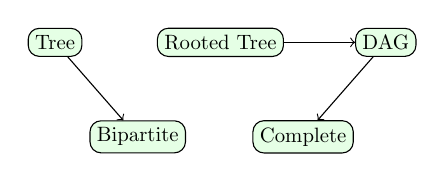
\begin{tikzpicture}[scale=0.75,every node/.style={transform shape}]
\node[draw,rounded corners,fill=green!10] (t) at (0,0.8) {Tree};
\node[draw,rounded corners,fill=green!10] (rt) at (2.8,0.8) {Rooted Tree};
\node[draw,rounded corners,fill=green!10] (dag) at (5.6,0.8) {DAG};
\node[draw,rounded corners,fill=green!10] (bi) at (1.4,-0.8) {Bipartite};
\node[draw,rounded corners,fill=green!10] (k) at (4.2,-0.8) {Complete};
\draw[->] (t)--(bi);
\draw[->] (rt)--(dag);
\draw[->] (dag)--(k);
\end{tikzpicture}
\end{frame}

\begin{frame}{기초 객체와 측도}
\begin{itemize}
  \item Degree: $\deg(v)$, Directed: $\deg^-(v),\deg^+(v)$
  \item Path, Cycle, Acyclic
  \item Centrality:
  \begin{itemize}
    \item Degree centrality
    \item Closeness centrality
    \item Betweenness centrality
  \end{itemize}
  \item Density:
\[
\rho_{\text{undir}}=\frac{|E|}{|V|(|V|-1)/2},\qquad
\rho_{\text{dir}}=\frac{|E|}{|V|(|V|-1)}
\]
\end{itemize}
\end{frame}

\begin{frame}{그래프 표현 방식 비교}
\begin{table}
\centering
\small
\begin{tabular}{lll}
\toprule
표현 & 장점 & 단점 \\
\midrule
Adjacency Matrix & 엣지 조회 $O(1)$ & 공간 $O(|V|^2)$ \\
Edge List & 저장 단순, 희소 그래프 유리 & 엣지 조회 느림 \\
Adjacency List & 공간 $O(|V|+|E|)$ & 엣지 조회는 Matrix보다 느릴 수 있음 \\
\bottomrule
\end{tabular}
\end{table}
\end{frame}

\begin{frame}{BFS vs DFS}
\begin{columns}
\begin{column}{0.5\textwidth}
\textbf{BFS}
\begin{itemize}
  \item Queue
  \item 레벨 순회
  \item 무가중치 최단경로 유리
\end{itemize}
\end{column}
\begin{column}{0.5\textwidth}
\textbf{DFS}
\begin{itemize}
  \item Stack/Recursion
  \item 깊이 우선 + 백트래킹
  \item 사이클 탐지/위상정렬 기반
\end{itemize}
\end{column}
\end{columns}
\vspace{0.3em}
\centering
시간복잡도: BFS/DFS 모두 $O(|V|+|E|)$
\end{frame}

\begin{frame}{Chapter 2 정리}
\begin{itemize}
  \item 그래프 성질: 방향성/가중치/연결성
  \item 그래프 유형: Tree, DAG, Bipartite, Complete
  \item 핵심 개념: Degree, Path, Centrality, Density
  \item 표현 방식과 탐색 알고리즘의 트레이드오프
\end{itemize}
\end{frame}

\section{마무리}
\begin{frame}{핵심 Takeaways}
\begin{enumerate}
  \item 그래프 학습의 본질은 관계 구조 활용
  \item GNN의 본질은 이웃 집계 기반 표현학습
  \item 그래프 이론(표현/탐색/측도)은 GNN 이해의 필수 기초
\end{enumerate}
\end{frame}




